\documentclass{sig-alternate}

\usepackage[utf8]{inputenc}
\usepackage[T1]{fontenc}
\usepackage{textcomp}
\usepackage[french, english]{babel}
\usepackage{graphicx}
\usepackage{url}
\usepackage{backnaur}
\usepackage{tikz}
\usepackage{xcolor}
\usepackage{color}
\usepackage{listings}
\usepackage{inconsolata}

\usepackage[hyperref=true,%
            url=false,%
            isbn=false,%
            style=numeric,%
            maxcitenames=3,%
            maxbibnames=100,%
            backend=bibtex,%
            block=none]{biblatex}
\bibliography{references.bib}

\definecolor{red}{rgb}{1,0,0.29}
\definecolor{green}{rgb}{0,0.91,0.75}
\definecolor{lightgray}{rgb}{.9,.9,.9}
\definecolor{gray}{rgb}{.6,.6,.6}
\definecolor{darkgray}{rgb}{.4,.4,.4}

\newcommand{\testbf}{bx}

\newcommand{\CodeSymbol}[1]{
    \bfseries\textcolor{red}{#1}
}

\newcommand\opstyle{\color{red}}

\lstdefinelanguage{js}{
  keywords={break, case, catch, continue, debugger, default, delete, do, else, false, finally, for, function, if, in, instanceof, new, null, return, switch, this, throw, true, try, typeof, var, void, while, with},
  morecomment=[l]{//},
  morecomment=[s]{/*}{*/},
  morestring=[b]',
  morestring=[b]",
  ndkeywords={class, export, boolean, throw, implements, import, this},
  keywordstyle=\color{red}\bfseries,
  ndkeywordstyle=\color{red}\bfseries,
  identifierstyle=\color{black},
  commentstyle=\color{lightgray}\ttfamily,
  stringstyle=\color{gray}\bfseries,
  basicstyle=\color{gray}\ttfamily\scriptsize,
  sensitive=true,
  escapeinside={\/\/\@}{\@}
}

\lstdefinelanguage{flx}{
  keywords={flx, fluxion},
  morecomment=[l]{//},
  morecomment=[s]{/*}{*/},
  morestring=[b]',
  morestring=[b]",
  literate= {+>}{{\ttfamily\scriptsize>>}}2
            {->}{{\CodeSymbol{->}}}2
            {>>}{{\CodeSymbol{>>}}}2, % This is a hack to get -> and >> be highlighted like keywords.
  ndkeywords={main, express\_dispatcher, app\_js, get, handler, reply, anonymous\_1000, null},
  keywordstyle=\color{red}\bfseries,
  ndkeywordstyle=\color{black}\bfseries,
  identifierstyle=\color{black},
  commentstyle=\color{lightgray}\ttfamily,
  stringstyle=\color{gray}\bfseries,
  basicstyle=\color{gray}\ttfamily\scriptsize,
  sensitive=true,
  escapeinside={\/\/\@}{\@}
}

\newcommand{\userlstset}[1]{
  \lstset{ %
    numberstyle=\tiny,               % the size of the fonts that are used for the line-numbers
    numbers=left,                    % where to put the line-numbers
    stepnumber=1,                    % the step between two line-numbers. If it is 1 each line will be numbered
    numbersep=5pt,                   % how far the line-numbers are from the code
    showspaces=false,                % show spaces adding particular underscores
    showstringspaces=false,          % underline spaces within strings
    showtabs=false,                  % show tabs within strings adding particular underscores
    tabsize=2,                       % sets default tabsize to 2 spaces
    captionpos=b,                    % sets the caption-position to bottom
    breaklines=true,                 % sets automatic line breaking
    breakautoindent = true,          %
    breakatwhitespace=false,         % sets if automatic breaks should only happen at whitespace
    escapeinside={\@}{\@},           % if you want to add a comment within your code
    language=#1,                     % choose the language of the code
  } %
}

\newcommand{\ic}[1]{\lstinline|#1|}

\lstnewenvironment{code}[1][js]{%
  \userlstset{#1}%
}{%
}

\newcommand{\includecode}[2]{%
  \userlstset{#1}%
  \lstinputlisting{#2}%
}

\newcommand{\ftnt}[1]{%
\footnote{\small{\url{#1}}}%
}

\newcommand*\circled[1]{%
  \tikz[baseline=(char.base)]{%
    \node[shape=circle,draw,inner sep=0.8pt] (char) {#1};%
  }%
}

\begin{document}

\title{
  Transforming Javascript Event-Loop Into a Pipeline
}

\numberofauthors{2}
\author{
\alignauthor
Etienne Brodu, Stéphane Frénot\\
  \email{\textsf{\normalsize{\{etienne.brodu, stephane.frenot\}@insa-lyon.fr}}}\\
  \affaddr{\textsf{\small{Univ Lyon, INSA Lyon, Inria, CITI, F-69621 Villeurbanne, France}}}
\and
\alignauthor
Frédéric Oblé\\
  \email{\textsf{\normalsize{frederic.oble@worldline.com}}}\\
  \affaddr{\textsf{\small{Worldline, Bât. Le Mirage, 53 avenue Paul Krüger}}}\\
  \affaddr{\textsf{\small{CS 60195, 69624 Villeurbanne Cedex}}}\\
}

\begin{CCSXML}
<ccs2012>
<concept>
<concept_id>10011007.10011006.10011041.10011047</concept_id>
<concept_desc>Software and its engineering~Source code generation</concept_desc>
<concept_significance>500</concept_significance>
</concept>
<concept>
<concept_id>10011007.10011006.10011041.10011048</concept_id>
<concept_desc>Software and its engineering~Runtime environments</concept_desc>
<concept_significance>500</concept_significance>
</concept>
</ccs2012>
\end{CCSXML}

\ccsdesc[500]{Software and its engineering~Source code generation}
\ccsdesc[500]{Software and its engineering~Runtime environments}

% \CopyrightYear{2016} %
% \setcopyright{licensedothergov} %
% \conferenceinfo{SAC 2016,}{April 04 - 08, 2016, Pisa, Italy \vspace{3pt}\\ %
% {\scriptsize Copyright is held by the owner/author(s). Publication rights licensed to ACM.}} %
% \isbn{978-1-4503-3739-7/16/04}\acmPrice{\$15.00} %
% \doi{http://dx.doi.org/10.1145/2851613.2851745} %

\maketitle

\begin{abstract}

The audience's growth of a web application is highly uncertain, it can increase and decrease in a matter of hours if not minutes.
This uncertainty often leads the development team to quickly adopt disruptive and continuity-threatening shifts of technology to handle the higher connections spikes.
% The audience's growth a web application needs to adapt to, often leads its development team to quickly adopt disruptive and continuity-threatening shifts of technology.
To avoid these shifts, we propose an approach that abstracts web applications into a high-level language, allowing code mobility to dynamically cope with audience growth and decrease.

We think a web application can be depicted as a network of small autonomous parts moving from one machine to another and communicating by message streams.
The high-level language we propose aims to express these parts and their streams.
We named these parts \textit{fluxions}, by contraction between a flux and a function.
\textit{Fluxions} are distributed over a network of machines according to their interdependencies to minimize overall data transfers.
We expect that this dynamic reorganization can allow an application to handle its load.

Our high-level language proposition consists of an execution model which dynamically adapts to the execution environment, and a tool to automate the technological shift between the classical model and the proposed one.

\end{abstract}

\printccsdesc
\keywords{Flow programming; Web; Javascript}

\eject

\section{Introduction}

\textit{``Release early, release often''}, \textit{``Fail fast''}.
The growth of a real-time web service is partially due to Internet's capacity to allow very quick releases of a minimal viable product (MVP).
% In a matter of hours, it is possible to release a prototype and start gathering a user community.
% \textit{``Release early, release often''}, and \textit{``Fail fast''} are the punchlines of the web entrepreneurial community.
It is crucial for the prosperity of such project to quickly validate that it meets the needs of its users.
Indeed, misidentifying the market needs is the first reason for startup failure\ftnt{https://www.cbinsights.com/blog/startup-failure-post-mortem/}.
Hence the development team quickly concretizes an MVP using a feature-driven approach and iterates on it.

% If the service successfully complies with users requirements, its community grows with its popularity.
The service needs to be scalable to be able to respond to the growth of its user-base.
However, feature-driven development best practices are hardly compatible with the required parallelism.
The features are organized in modules which disturb the organization of a parallel execution \cite{Clements2013a,Hughes1989,Parnas1972}.
Eventually the growth requires to discard the initial approach to adopt a more efficient processing model.
Many of the most efficient models decompose applications into execution units \cite{Fox1997, Welsh2000, Dean2008}.
% This decomposition may be spread over a cluster of commodity machines \cite{Fox1997}.
% MapReduce \cite{Dean2008} and the Staged Event-driven Architecture (SEDA) \cite{Welsh2000} are famous examples of that trend. %, using a pipeline architecture.
% Once split, the service parts are connected by an asynchronous messaging system.
% Many tools have been developed to express and manage these service parts and their communications.
% We can cite Spark \cite{Zaharia2012}, MillWheel \cite{Akidau2013}, Naiad \cite{McSherry}, Storm \cite{Toshniwal2014}, and many others.
However, these tools are in disruption from the initial approach.
% It requires the development team either to be trained or to hire experts, and more importantly, to start over the initial code base.
This shift causes the development team to spend development resources in background to start over the initial code base, without adding visible value for the users.
It is a risk for the evolution of the project.
Running out of cash and missing the right competences are the second and third reasons for startup failures$^2$.
% \ftnt{https://www.cbinsights.com/blog/startup-failure-post-mortem/}

The risk described above comes from a disruption between the two levels of application expression, the feature level and the execution level.
To avoid this risk and allow a continuous development process, we propose a tool to automatically map one level onto the other, and make the transition.
% , and allow an automatic transition from one to the other and back.
% we propose a tool to identify an alignment between the two levels, so as to allow a continuous transition from one to the other and back.
% This compiler transforms the initial code base into a high-level language.
% in the application allowing parallelism, hence scalability.
% This tool should allow a continuous development process.

We focus on web applications driven by users requests and developed in Javascript using the \textit{Node.js}\ftnt{https://nodejs.org/} execution environment.
% It is the most used language on Github\ftnt{http://githut.info/} and StackOverflow\ftnt{http://stackoverflow.com/tags}.
Javascript is widely adopted\ftnt{http://githut.info/}\ftnt{http://stackoverflow.com/tags} to develop web applications, and its event-loop model is very similar to a pipeline architecture.
% think that it is possible to identify the stages of this pipeline in an application. % a stream of requests passing through a pipeline
% Indeed, the event-loop used in \textit{Node.js} is very similar to a pipeline architecture.
% We 
So we propose a compiler to transform an application into a pipeline of parallel stages communicating by message streams.
We named these stages \textit{fluxions}, by contraction between a flux and a function.

% The contribution of this paper are the identification and partial resolution of the problems arising from the isolation of the global memory into fluxions.
% Second, a partial resolution of these problems, allowing an experimental compilation.
% We are interested in the problems arising from the isolation of the global memory into these fluxions.
%T his tool and its runtime aim not to modify the existing code, but rely on a high-level language expression over the initial code base.
% The contribution of this paper is the resolution of these problems, allowing the compilation.
We present a proof of concept for this compilation approach.
Section \ref{section:model} describes the execution environment targeted by this compiler.
Then, section \ref{section:compiler} presents the compiler, and section \ref{section:evaluation} its evaluation.
Section \ref{section:related} compare our work with related works.
And finally, we conclude this paper.
\section{Fluxional execution model} \label{section:model}

Many frameworks for distributed systems are renowned for their performances\cite{Welsh2000, Jain2006, Wu2007, Zaharia2010, Akidau2013, Marz2011}.
However, we focus on a compilation approach to replace the shift in programming model rather than the performance of the runtime.
We present in this section an extremely simplified but generic execution model inspired by the literature, only to support the confirmation of feasibility for the compilation process detailed in section \ref{section:compiler}.
The execution model is not distributed on remote machines, however it isolates the execution of fluxions in different process to reproduce the execution conditions of a distributed execution model.
We are interested in the problems arising from this isolation.

\subsection{Fluxions and workers}

The fluxional execution model manages and invokes autonomous execution units named fluxion $\bnfpn{flx}$.
A fluxion is composed of a unique name $\bnfpn{id}$, a processing function $\bnfpn{fn}$, and a persisted memory called a \textit{context} $\bnfpn{ctx}$.
It is a function $\bnfpn{fn}$ consuming an input stream $\bnfpn{stream}$ and generating one or more outputs streams to other fluxions $\bnfpn{dest}$.
It listens for, and sends back continuous sequence of messages.
The \textit{context} persists the state on which a fluxion rely between two message receptions.
At a message reception, the fluxion modifies its \textit{context}, and sends back messages to downstream fluxions.
A message is composed of the recipient fluxions' names and a body.

Fluxions are executed on workers.
A worker is an event-loop and an isolated heap ; it is a \textit{Node.js} instance.

The context of a fluxion is lexically isolated.
It has a distinct lexical scope containing variables not shared with any other fluxion.
Fluxions on the same worker share the same event-loop, and the same heap ; they send references to each over.
Fluxions on different workers have different event-loop and heaps ; their communications are serialized, so it impossible to send heap references.
The event-loop assures the exclusivity and atomicity of operations of each fluxion on the heap.
This organization shows that the more the memory is shared, the harder it is to distribute fluxions on different workers to allow parallelisation of their execution.

We represent here the syntax of a high-level language to represent a program in the fluxionnal form.
It is the target for our compiler.

\begin{bnf*}
  \bnfprod{program}    {\bnfpn{flx} \bnfor \bnfpn{flx} \bnfsp \bnftd{eol} \bnfsp \bnfpn{program}}\\
  \bnfprod{flx}        {\bnfts{\texttt{flx}} \bnfsp \bnfpn{id} \bnfsp \bnfpn{ctx} \bnfsp \bnfpn{worker} \bnfsp \bnftd{eol} \bnfsp \bnfpn{streams} \bnfsp \bnftd{eol} \bnfsp \bnfpn{fn}}\\
  \bnfprod{worker}     {\bnfts{\texttt{on}} \bnfsp \bnfpn{id} \bnfor \bnftd{empty string}}\\
  \bnfprod{streams}    {\bnfts{\texttt{null}} \bnfor \bnfpn{stream} \bnfor \bnfpn{stream} \bnfsp \bnftd{eol} \bnfsp \bnfpn{streams}}\\
  \bnfprod{stream}     {\bnfpn{op} \bnfsp \bnfpn{dest} \bnfsp [\bnfpn{msg}]}\\
  \bnfprod{dest}       {\bnfpn{list}}\\
  \bnfprod{ctx}        {\bnfts{\texttt{\{}} \bnfpn{list} \bnfts{\texttt{\}}}}\\
  \bnfprod{msg}        {\bnfts{\texttt{[}} \bnfpn{list} \bnfts{\texttt{]}}}\\
  \bnfprod{list}       {\bnfpn{id} \bnfor \bnfpn{id} \bnfsp \bnfts{,} \bnfsp \bnfpn{list}}\\
  \bnfprod{op}         {\bnfts{\texttt{>}\texttt{>}} \bnfor \bnfts{\texttt{-}\texttt{>}}}\\
  \bnfprod{id}         {\bnftd{Javascript identifier}}\\
  \bnfprod{fn}         {\bnftd{Javascript and stream syntax}}\\
\end{bnf*}
\vspace{-1.5\baselineskip}~\\

Fluxions are the stages in a pipeline architecture.
The streams of messages between fluxions are carried by the messaging system.

\subsection{Messaging system}

In a distributed approach, the messages between fluxions would be carried over a distributed message broker.
But because this execution model intends only to simulate a distributed execution environement, we simplify a distributed message broker with a centralised message queue.
% The messaging system is the core of the execution model.
% It carries messages and invokes fluxions at reception.
The messaging system sends messages to the isolated worker hosting the destination fluxion.
The worker containing the messaging system is itself a worker, and contains locally fluxion that cannot be isolated from the network interfaces.
% Using a message queue allows to execute multiple processing chains fairly and concurrently, without difference in scheduling local messages, or network messages.
The life cycle of a fluxional application is illustrated in figure \ref{fig:MesSys}.

\begin{figure}[h!]
  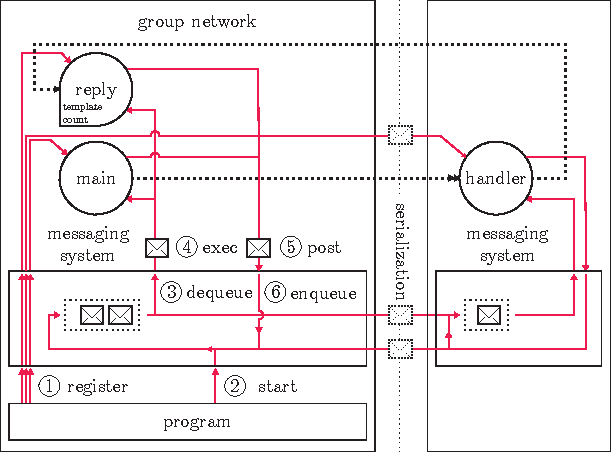
\includegraphics[width=\linewidth]{ressources/schema-message.pdf}
  \caption{Messaging system details}
  \label{fig:MesSys}
\end{figure}

The messaging system carries messages based on the names of the recipient fluxions.
If two fluxions share the same name, it would lead to a conflicting situation for the messaging system.
Every fluxion needs to be registered with a unique name.
This registration associates a processing function with a unique name and an initial \textit{context}.
The registration is done using the function \texttt{register(<name>, <fn>, <context>)}, \circled{1}.
% A fluxion can dynamically register other fluxions

To trigger a chain of fluxions, a message is sent using the function \texttt{start(<msg>)}, \circled{2}.
This first message represent the incoming of a request from a user.
% This function pushes a first message in the queue.
The system dequeues this message and dispatch it to the destination fluxion, \circled{3} and \circled{4}.
The recipient function sends back messages from the isolated worker using the function \texttt{post(<msg>)}, \circled{5}, to be enqueued in the centralised message queue, \circled{6}.
The system loops through steps \circled{3} and \circled{4} until the queue is empty.
This cycle starts again for each new incoming request causing a \textit{start} message.

Algorithms \ref{alg:parcours} and \ref{alg:traitement} describe the behavior of the messaging system after the \texttt{start} function invocation.

\begin{algorithm}
\caption{Message queue walking algorithm}
\label{alg:parcours}
\begin{algorithmic}
\Function{loopMessage}{\null}
\While{$msg$ \textbf{presents in} $msgQueue$}
\State $msg \gets$ \Call{dequeue}{\null} \Comment{\circled{3}}
\State \Call{ProcessMsg}{$msg$}
\EndWhile
\EndFunction
\end{algorithmic}
\end{algorithm}

\begin{algorithm}
\caption{Message processing algorithm}
\label{alg:traitement}
\begin{algorithmic}
\Function{processMsg}{$msg$}
\For{$dest$ \textbf{in} $msg.dest$}
\State $worker \gets lookup(dest)$
\State \Call{worker.send}{$fluxion, msg.body$} \Comment{\circled{4}}
% \State $message \gets$ \Call{exec}{$fluxion, msg.body$} \Comment{\circled{4} \& \circled{5}}
% \State \Call{enqueue}{$message$} \Comment{\circled{6}}
\EndFor
\EndFunction
\end{algorithmic}
\end{algorithm}

\subsection{Service example}

To illustrate the fluxional execution model, and the compiler we present an example of a simple web application.
This application reads the file containing its own source code, and sends it back along with a request counter.

The original source code of this application is available on github\cite{flx-example}, and in listing \ref{lst:source}.
In this source code, some points are worth noticing.

\begin{itemize}
  \item The \texttt{handler} function, line 5 to 11, contains the logic we want to split into the fluxional processing chain.
  It receives the user request in the variable \texttt{res} which is used by the last function of the chain, \texttt{reply}.
  \item The \texttt{count} object at line 3 is a persistent memory that increments the request counter.
  This object needs to be mapped to a fluxion \textit{execution context} in the fluxional execution model.
  \item The \texttt{app.get} and \texttt{app.send} methods, respectively line 5 and 9, interface the application with the clients.
  The processing chain of functions occurs between these two functions : $\texttt{get} \twoheadrightarrow \texttt{handler} \to \texttt{readFile} \to \texttt{reply} \to \texttt{send}$.
\end{itemize}

\includecode{js,
  caption={Simple web application. \textnormal{this application replies to every user request with its own source code and the value of a request counter}},
  label={lst:source}
}
{../../flx-example/source.js}

This application is transformed manually into the fluxions chain depicted in Figure \ref{fig:fluxions}.
We expect a similar result with the compiler described in section \ref{section:compiler}.
Circles represent registered fluxions.
Envelope symbols represent messages streams between fluxions with the variables transmitted from one fluxion to the other.
The square in the messaging system holds the \textit{context} of the \texttt{reply} fluxion.
When a new REST request \texttt{GET} is received, a \texttt{start} message triggers the flow.
The \texttt{handler} fluxion receives this \texttt{start} message, reads the source file and forwards it to the \texttt{reply} fluxion which increments the counter, and sends the result back.
Each fluxion propagates the necessary values from one fluxion to the other exclusively by messages.
Horizontal dashed lines show virtual transmission of messages between fluxions although they all go through the messaging system.

\begin{figure}[h!]
  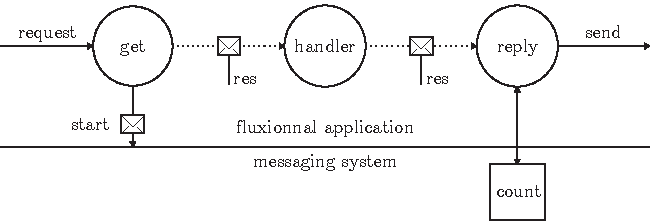
\includegraphics[width=\linewidth]{ressources/flux.pdf}
  \caption{Fluxions chain manually extracted from the example application}
  \label{fig:fluxions}
\end{figure}

\begin{code}[flx, caption={Manual transformation of the example application in our high-level fluxional language},label={lst:fluxional}]
flx get
>> handler [res]
  var app = require('express')(),
      fs = require('fs'),
      count = 0;

\\@\label{lst:fluxional-streamtohandler}@  app.get('/', >> handler);
  app.listen(8080);
  console.log('>> listening 8080');

flx handler
-> reply [res]
  function handler(req, res) {
\\@\label{lst:fluxional-readfile}@      fs.readFile(__filename, -> reply);
  }

flx reply {count}
-> null
  function reply(error, data) {
\\@\label{lst:fluxional-counter}@    count += 1;
    var code = ('' + data).replace(/\n/g, '<br>').replace(/ /g, '&nbsp');
\\@\label{lst:fluxional-ressend}@    res.send('downloaded ' + count + ' times<br><br><code>' + code + '</code>');
  }
\end{code}

The application is organized as follow :
\begin{itemize}
  \item The \texttt{get} fluxion is the \textit{root} fluxion.
  It initializes the application to listen for user requests by calling \texttt{app.get}.
  Every request is forwarded on the stream to the \texttt{handler} fluxion, line \ref{lst:fluxional-streamtohandler}.
  \item The \texttt{handler} fluxion reads the file containing the source code of the application, and forwards the result to the \texttt{reply} fluxion, line \ref{lst:fluxional-readfile}.
  \item The \texttt{reply} fluxion increments the counter, line \ref{lst:fluxional-counter}, formats the reply, and sends it back to the user using the function \texttt{res.send}, line \ref{lst:fluxional-ressend}.
\end{itemize}

Our goal, as described in the introduction, is not to propose a new programming paradigm with this high-level language but to automate the architecture shift with a compiler.
\section{Designing a compiler for fluxional compliancy} \label{section:compiler}

% The section \ref{section:model} of this paper describes the fluxional execution model, a framework to run web application in a distributed environment.
% This section explains the compiler we developed to transform a subset of classic web application to be compliant with the execution model previously described.
% This transformation unveils two problems due to the differences between a web application and the execution model.
% In the first section, a distributed system is defined by the parallel execution of its parts, and the distribution of its memory.
Current Web applications are mostly written in Java. The langage proposes both data encapsulation and a threading model that ease the development of distributed applications.
Yet, Java framework for developing efficient applications are complex systems that impose new APIs\cite{Coward2003} to the developers.
They are error-prone, and leads to deadlocks and other synchronization problems.
Since 2009, \textit{Node.js}\cite{Dahl} provides a simple Javascript execution environnment for network applications.
We focus on this promising environment for its initial simplicity and efficiency.
We develop a compiler that transforms a simple \textit{Node.js} application into a fluxional system compliant to the architecture described in section \ref{section:model}.
As javascript forbids user-space thread API, a javascript application is developed as a mono-threaded application.
Moreover, in Javascript  the memory is hierarchical and the root scope may be accessed by any function, which leads to bad component isolation.
Our compiler uses a new approach to find rupture points into most of \textit{Node.js} application, marking out the independent application pars.
It assures isolation and memory consistency for the application parts.

We do not target all Javascript Web-based application as this work is only a proof of concept of the compilation process.
But if we are able to transform a consequent subset of currently running applications without external developer help, we expect a real execution gain in a cloud environment.
The rest of this section describes the two parts of the compiler responsible to isolate application parts.
Section \ref{section:analyzer} explains how the \textit{analyzer} detects rupture points in the web application to mark out the independent parts.
Section \ref{section:linker} explains how the \textit{linker} resolves the missing dependencies due to the distribution of the central memory.

% TODO move this
% The compiler reuses some tools from the Javascript community.
% The compiler and these tools follow the specification for an intermediate representation of the Javascript source code from the Mozilla Javascript Parser API\cite{JsAST}.
% \textit{Esprima}\cite{esprima} parses the source and generate an Abstract Syntax Tree (AST).
% The compiler analyze and modify this tree by traversing it using \textit{Estraverse}\cite{estraverse}.
% \textit{Escope}\cite{escope} extracts function scopes and variables declaration from the tree.
% At the end of the compilation chain, the compiler uses \textit{Escodegen}\cite{escodegen} to transform AST back into Javascript source code.

\subsection{Analyzer : execution parallelism} \label{section:analyzer}

% The parallelization of programs is a trending problem to leverage the multiple cores available on highly parallel architectures.
The Sun programming guide\footnote{\raggedright http://docs.oracle.com/cd/E19455-01/806-5257/6je9h032b/index.html} defines \textbf{parallelism} as \textit{a condition that arises when at least two threads are executing simultaneously}, and \textbf{concurrency} as \textit{a condition that exists when at least two threads are making progress. A more generalized form of parallelism that can include time-slicing as a form of virtual parallelism}.
\textbf{Asynchronism} is a condition that arises when a client continues its execution while waiting for the result to its request.

Promises\cite{Liskov1988}, as well as callbacks, are abstractions that transform blocking synchronous operations into non-blocking asynchronous operations.
These asynchronous operations run in parallel with the main thread, until the requested result is available for the main thread to continue the computation needing this value.
The callback asynchronism splits the execution in two concurrent execution paths, one that needs the requested result and one that doesn't.
A rupture points is where the execution flow forks in two concurrent paths due to this asynchronism.
These points mark out the limits between the independent parts of an application.
 
The analyzer detects rupture points to break the application into independent parts.
In this section, we define what a rupture point is, and how the compiler detects them.

\subsubsection{Rupture points}

Rupture points represent a fork in the execution flow due to an asynchronous operation.
They are composed of an asynchronous function, and a callback to process the result of the operation.
The first execution flow path is the suite of instructions following after the asynchronous function.
The second execution flow path is the callback.
A rupture point is an interface between these two execution flows and split them in two application parts.
Listing \ref{lst:hello} is an example of a rupture point in a simple application.
The asynchronous function call \texttt{fs.readFile} and the callback \texttt{function display} represent the rupture point between the first execution path, line \ref{lst:first_ep} and the second, line \ref{lst:second_ep}.
The first application part is the whole program, the second application part contains the \texttt{function display}, lines \ref{lst:callback_begin} to \ref{lst:callback_end}.

\begin{code}[js, caption={Example of a rupture point : an asynchronous function call, \texttt{fs.readFile()}, with a callback parameter, \texttt{function display}},label={lst:hello}]
var fs = require('fs');

@\label{lst:callback_begin}@fs.readFile(__filename, function display(err, data) {
@\label{lst:second_ep}@  console.log('>> second concurrent execution path');
  console.log(err || data.toString());
@\label{lst:callback_end}@})

@\label{lst:first_ep}@console.log('>> first concurrent execution path');
\end{code}

\begin{figure}[h!]
\begin{center}
  \includegraphics[width=\linewidth]{ressources/flux-1.pdf}
  \caption{Division of the listing \ref{lst:hello} into two application parts}
  \label{fig:flux-1}
\end{center}
\end{figure}

There are two types of rupture points : \textit{start} and \textit{post}.
Figure \ref{fig:basicrp} and \ref{fig:specialrp} illustrate the different types of interface in the rupture points.
In these figures, the two concurrent execution paths are indicated by \circled{1} and \circled{2}, the applications parts are encapsulated in upstream and downstream fluxions.

\textbf{Start rupture points} are on the interface between the whole application and the outside, continuously receiving incoming user requests, like \texttt{app.get()} in listing \ref{lst:rupturepoints}.
These functions indicate the input of a data stream in the program, and the beginning of a chain of application parts following this stream.
% The \textit{start} rupture points will later be used to monitor the load from incoming external requests.
The asynchronous function is called only once, while the callback is triggered for each new request.
The interface of this rupture point is placed between the two, as illustrated in figure \ref{fig:basicrp}, because it is a convenient separation between two functions.

\textbf{Post rupture points} represent a continuity in the execution flow after a finite asynchronous operation, such as reading a file in listing \ref{lst:hello}.
As the result of this read operation probably being a voluminous object, this frontier is specially placed before the call to the asynchronous function, but after the resolution of the arguments.
This placement allow the asynchronous function call to occur in the same application parts as the callback, avoiding the transfer of this voluminous result, as illustrated in figure \ref{fig:specialrp}.
% The function calls from following rupture points mark the interface between the current application part and the next one.
For a write operation, the data transfer is inversed so the frontier is placed between the asynchronous operation and the callback, like for a \textit{start rupture point}, as illustrated in figure \ref{fig:basicrp}.

\begin{figure}[h!]
\begin{center}
  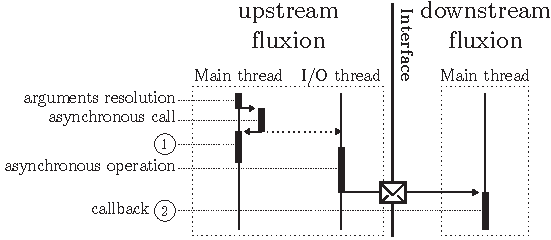
\includegraphics[width=\linewidth]{ressources/basicrp.pdf}
  \caption{Basic rupture point interface. \textnormal{The rupture point interface is placed after the asynchronous operation, for the downstream application part to be triggered at each event.}}
  \label{fig:basicrp}
\end{center}
\end{figure}

\begin{figure}[h!]
\begin{center}
  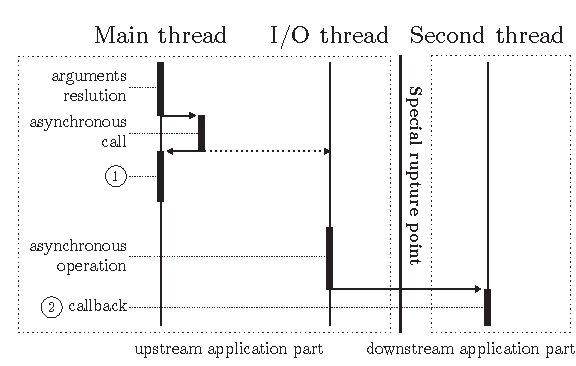
\includegraphics[width=\linewidth]{ressources/specialrp.pdf}
  \caption{Special rupture point interface. \textnormal{The rupture point interface is placed before the asynchronous operation, to avoid moving the result accross the interface from one application part to the other.}}
  \label{fig:specialrp}
\end{center}
\end{figure}

\begin{code}[js, caption={Example of an application presenting the two types of rupture points : a \texttt{start} with the call to \texttt{app.get()}, and a \texttt{post} with the call to \texttt{fs.readFile()}},label={lst:rupturepoints}]
var app = require('express')(),
    fs = require('fs');

app.get('/', function handleRequest(req, res) {
  fs.readFile(__filename, function reply(err, data) {
    res.send(err || data.toString());
  })
});

app.listen(8080);
console.log('server listening to 8080');
\end{code}

\begin{figure}[h!]
\begin{center}
  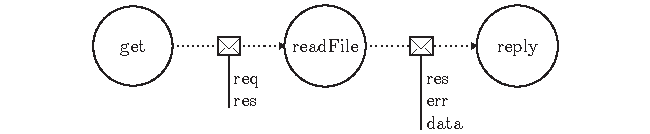
\includegraphics[width=\linewidth]{ressources/flux-2.pdf}
  \caption{Division of the listing \ref{lst:rupturepoints} into three application parts}
  \label{fig:flux-1}
\end{center}
\end{figure}

\subsubsection{Detection}

Detecting a rupture point requires detecting its two components : the asynchronous function and the callback function.

\textbf{Asynchronous functions}\\
The compiler is prebuilt knowing some module names exposing asynchronous function, like the \textit{express}, and the \textit{fs} module in listing \ref{lst:rupturepoints}.
To detect asynchronous calls, the compiler keep a list of variables holding such modules, to later detects their asynchronous function calls.
In listing \ref{lst:rupturepoints}, the compiler adds both variables \texttt{app} and \texttt{fs} in this list.
When the compiler encounter a call expression, it compare its callee name with this list to spot asynchronous functions.

\textbf{Callback function}\\
For each asynchronous call expression detected, the compiler test if one of the arguments is of type \texttt{function} to spot the callback.
Some callback functions are declared \textit{in situ}, and are trivially detected.
For every other variable identifier, we track the declaration up to the initialization value to detect its type.

\textbf{Variable tracking}\\
To detect both the asynchronous function and the callback function, the compiler needs to statically track the types of variables.
Missing rupture points by false negatives in the detection is sub-optimal, but false positives are more critical, as it eventually produces a runtime execution.
Therefore, the detection needs to be as accurate as possible to screen out false positives.
We use a technique similar to a Program Dependency Graph (PDG)\cite{Ferrante1987} to track changes in the value of variables.


\subsection{Linker : memory distribution} \label{section:linker}

% Because of the central memory, parallelism is not sufficient for an application to be distributed.
Parallelism is not enough for an application to be distributed.
The compiler also needs to distribute the memory into the application parts for the application to be compliant with the fluxional execution model.
In Javascript, scopes are nested one in the other up to the all-enclosing global scope.
Each function creates a new scope containing variables local to itself, and chained to the scope of the parent function.
% The child function can access variables in the scope of the parent functions, up to the global scope.
Rupture points always take place in between scopes, linking application parts in message streams.
A rupture point placed between a child scope and its parent breaks a chain of scope, and makes the child unable to access its parent as expected, eventually leading the application to runtime error.
The linker analyzes how scopes are distributed among the application parts to detect and resolve unmet dependencies between them.
Depending on how a shared variable is used in the scopes, there are different situations to resolve.
In the following, we explain the different cases of inconsistency emerging from the partitioning of a central memory.

\subsubsection{Signature}

The signature is the part of a message containing all the variables to send downstream, like the variable \texttt{res} in figure \ref{}\TODO.
If a variable is needed for read-only access by at least one downstream application part, it is added to the signature of the rupture point.
As fluxions are chained one after another, a fluxion must provide every dependency for the next one, even if some of this dependencies are not needed by the current application part.
These dependencies must be passed fluxion after fluxion from the producing fluxion to the consuming fluxion.
The compiler modifies those variable identifiers inside the application part to make them point to the message signature instead of the function scope.

\subsubsection{Scope}

% The scope is the name given to the persisted memory of a fluxion.
The scope of an application part consist of all the variables declared outside, but needed for modification in only this application part.
If one of these variables needs to be read by another application part downstream, this variable also becomes part of the signature sent downstream.
An example of such a variable is the \texttt{counter} in listing \ref{lst:ex-source}. Initialized to 0 in the global scope, the counter is incremented for each request by the \texttt{function reply}.
This counter is in the scope of the application part containing \texttt{function reply}.
The scope of an application part is stored in the context of the encapsulating fluxion.

\subsubsection{Sync}

If a variable is needed for modification by more than one distributed application parts, this variable needs to be synchronized between the fluxions.
The synchronization of a distributed memory is a well-known subject, with Brewer's theorem\cite{Gilbert2002}\cite{codahale2010}, and the ACID (Atomicity, Consistency, Isolation, Durability) versus BASE (Basically Available, Soft state, Eventual consistency) opposition\cite{Fox1997}.
We choose to stay out of this topic, the objective for this compiler is to be able to transform only a subset of web application with a satisfying result.
The compiler merges the parts too tightly coupled by modification accesses on a shared variable.

\subsection{Compilation example}

% For copyright reason, the compiler source code is kept private along with the tests we used.
To illustrate the compiler features, we compiled the illustration application used in section \ref{model}.
The source and compiled results of this application are available on github\cite{flx-example}\footnote{\raggedright https://github.com/etnbrd/flx-example/releases}.
The compiler source code is the property of Worldline, and is not publicly available, but we are planning of releasing it as an open source project in a near future.

To test the source or the result of the compilation, one would launch respectively \texttt{source.js} or \texttt{result.js} with \texttt{node} and check the service available at \texttt{localhost:8080}.
Both executable needs their dependencies to be resolved with \texttt{npm} before execution.
\begin{verbatim}
git clone https://github.com/etnbrd/flx-example
cd flx-example
npm install
node result.js
open http://localhost:8080
\end{verbatim}

The file \texttt{source.js}, in listing \ref{lst:ex-source}, is the source of this compilation example.
This application sends back its own source along with a download counter.
The processing chain of function is : $\texttt{get} \to \texttt{handler} \to \texttt{readFile} \to \texttt{reply} \to \texttt{send}$.
It uses two asynchronous function call with \textit{in situ} callback, one to listen for user requests and one to read its own source, respectively \texttt{app.get} line 5 and \texttt{fs.read} line 6.
It uses a global variable to increment the download counter defined line 3.
This global variable is used only in the \texttt{reply} function, line 7 and 9.

\includecode{js,
  caption={Source of the compilation example},
  label={lst:ex-source}
}
{../../example/source.js}

The result of the compilation into our high-level language is in the file \texttt{result.flx}, presented in listing \ref{lst:ex-flxres}.
The analyzer detects both asynchronous calls as rupture points.
The first one is a \textit{start} rupture point, associated with the \texttt{app.get} asynchronous function call which makes the callback \texttt{handler} listen for the stream of user requests. 
The second one is a \textit{post} rupture point, associated with the \texttt{fs.readFile} asynchronous function call which reads the source file and hands it to the callback \texttt{reply}.
These two rupture points result in three application parts.
The first application part is encapsulated in the root fluxion, named after the filename, \texttt{source.js}, line 18.
It initializes the system to route the user requests to the fluxion \texttt{handler-1000}, line 9.
This second fluxion reads the file, and sends the result to the next and last fluxion \texttt{reply-1001}, line 1.
We can identify the processing chain of functions in this chain of fluxion.

\begin{center}
\texttt{source.js} (\texttt{get})\\
$\downarrow$\\
\texttt{handler-1000} (\texttt{handler}, \texttt{readFile})\\
$\downarrow$\\
\texttt{reply-1001} (\texttt{reply}, \texttt{send})
\end{center}

The linker detects that the fluxion \texttt{reply-1001} needs two variable to send the result back to the user, \texttt{res} and \texttt{count}, as seen line 10 in listing \ref{lst:ex-flxres}.
The variable \texttt{res} depends on the user connection and is initialized for each new request.
It needs to be part of the \textit{signature} of the message transfered to the last fluxion.
The variable \texttt{count} is global, and the function \texttt{reply} in the fluxion \texttt{reply-1001} needs to increment it at each new request.
This global variable is in the scope of only this application part, so the compiler stores it in the context of this fluxion.

\includecode{flx,
  caption={High level fluxional language result of the compilation example},
  label={lst:ex-flxres}
}
{../../example/result.flx}

The compiler also produces an executable targeting an simple implementation of the fluxional execution model.
This result is in the file \texttt{result.js}, presented in listing \ref{lst:ex-jsres}.
The root fluxion is not registered because it doesn't need to receive any messages by another fluxion, it only initializes the application.
The two following fluxions are registered in the messaging system.
This registration encapsulates the processing function in a \texttt{function capsule}.
The special rupture points implies the asynchronous call to be in the downstream fluxion.
The \texttt{function capsule} encapsulates the asynchronous call from special rupture points or callbacks from basic rupture points in a unified processing function.
Line 3, the original callback is replaced with a \texttt{function placeholder}, sending the \textit{start} message to the fluxion \texttt{handler-1000}.
Line 17, the fluxion \texttt{handler-1000} pushes the user request \texttt{res} in the message and \texttt{post} it directly to the next fluxion, \texttt{reply-1001}.
Because there is a special rupture point between the fluxion \texttt{handler-1000} and \texttt{reply-1001}, the asynchronous call is moved to the next fluxion and the \texttt{function post} doesn't replace the callback.
Finally, the fluxion \texttt{reply-1001} receives the message containing the user request and read the file.
The callback of this asynchronous operation, line 27, increments the variable \texttt{counter}, line 28, and sends the reply, line 30.

\includecode{flx,
  caption={Fluxional execution model result of the compilation example},
  label={lst:ex-jsres}
}
{../../example/result.js}

\subsection{Limitations}

This compiler aims at transforming a subset of Javascript web applications presenting a specific syntax and design.
In this section, we describe briefly the current limitations of our compiler and how we plan to overcome them in future works.

\begin{itemize}
  \item Variables poorly encapsulated or used too broadly tighten dependencies accross the code, and might result in a coarser division of the application.
  \item The compilation silently fails if a variable holding a callback or a module is overwritten, or not defined in the declaration.
        The variable tracker is unable to track accurately all the modification of a variable to detect this situation which may lead the compiler either to miss rupture points, or to detect non existing one.
  \item The compiler is unable to track a dynamically resolved value, even if the value is deducible statically.
        If this variable is used in a potential rupture point, the compiler screens it out.
  \item The Javascript language offers rich composition possibilities leading to many corner cases.
        The compiler is not robust enough to understand all corner cases.
        For example, the \textit{express} module is only detected if initialized like in listing \ref{lst:rupturepoint}.
\end{itemize}
There may be other limitations we aren't aware of.

The three last limitations described above are caused by the variable tracker - described in section \ref{section:analyzer} - being in an early stage of development.
We are currently in the process of improving the robustness of the compiler to extend the subset of compilable applications.

% We believe that our work will keep scalability concerns out of the way for the development team, who could then focus on the core logic of their application.
% In future developments of this project, we aim at making application dynamically reactive to the load of user requests.
% By monitoring only the input stream, the \texttt{start} rupture points, we believe it is possible to infer the load propagation through the application.
% Using analogy with fluid dynamics, each fluxion is like a pipe, traversed by a fluid of user requests.
% The input and output throughput of this pipe could be calibrated before production use, generating an approximative model of the application reaction to input load.
% Using this model, we want to make the application's reorganize itself in a cluster to handle pikes in the user request throughput.

\section{Real case test} \label{section:evaluation}

The goal of this evaluation is to prove the possibility for an application to be compiled into a network of independent parts.
We want to show the current limitation of this isolation and the modification needed on the application to circumvent these limitations.
% TODO -> and finally, we present the possibilities of future works.
% We want to show the limitations of this isolation for future works, and the modifications needed to circumvent these limitations.

For brevity, we present in this paper only one test on a real application, gifsockets-server\ftnt{https://github.com/twolfson/gifsockets-server}.
% This application is part of the selection from our previous paper \cite{Brodu2015}.
% We chosed it because it is a working application, simple enough to illustrate this evaluation.
This application was selected from the \texttt{npm} registry because it depends on \texttt{express}, it is tested and working, and it simple enough to illustrate this evaluation.

This application is an example of a real-time chat using gif-based communication channels.
The client sends a request containing a text typed by the user.
The server transforms this text into a gif frame, and pushes this frame back to a never-ending gif to be displayed on the client.
Listing \ref{lst:gifsocket} is a simplified version of this application, containing only essential lines.

% The web application framework used in this application, \textit{express}, allows to register chains of functions to process user requests.
On line \ref{lst:gifsocket:app.post}, the application registers two functions to process the requests received on the url \texttt{/image/text}.
The closure \texttt{saveBody}, line \ref{lst:gifsocket:saveBody}, returned by \texttt{bodyParser}, line \ref{lst:gifsocket:bodyParser}, and the method \texttt{routes.write\-Text\-To\-Images} from the external module \texttt{gifsockets-middleware}, line \ref{lst:gifsocket:gif-mw}.
The closure \texttt{saveBody} calls the asynchronous function \texttt{getRawBody} to get the request body.
Its callback handles the errors, and calls \texttt{next} to continue the execution with the next function, \texttt{routes.write\-Text\-To\-Images}.

% The closure \texttt{saveBody} gather the whole request, and let \textit{express} call the next function in the chain, \texttt{routes.write\-Text\-To\-Images}, by calling \texttt{next}, line \ref{lst:gifsocket:next}.

\begin{code}[js, caption={Simplified version of gifsockets-server},label={lst:gifsocket}]
var express = require('express'),
    app = express(),
    routes = require('gifsockets-middleware'); //@\label{lst:gifsocket:gif-mw}@
    getRawBody = require('raw-body');

function bodyParser(limit) { //@\label{lst:gifsocket:bodyParser}@
  return function saveBody(req, res, next) { //@\label{lst:gifsocket:saveBody}@
    getRawBody(req, { //@\label{lst:gifsocket:getRawBody}@
      expected: req.headers['content-length'],
      limit: limit
    }, function (err, buffer) { //@\label{lst:gifsocket:callback}@
      % // If there was an error (e.g. bad length, over length), respond poorly
      % if (err) {
      %   res.writeHead(500, {
      %     'content-type': 'text/plain'
      %   });
      %   return res.end('Content was too long');
      % }
      req.body = buffer;
      next(); //@\label{lst:gifsocket:next}@
    });
  };
}

app.post('/image/text', bodyParser(1 * 1024 * 1024), routes.writeTextToImages); //@\label{lst:gifsocket:app.post}@
app.listen(8000);
\end{code}


\subsection{Compilation}

We compile this application with the compiler detailed in section \ref{section:compiler}.
% The function \texttt{getRawBody}, line \ref{lst:gifsocket:getRawBody}, is asynchronous.
The function call \texttt{app.post}, line \ref{lst:gifsocket:app.post}, is a rupture point.
However, its callbacks, \texttt{bodyParser} and \texttt{routes.write\-Text\-To\-Images} are evaluated as function only at runtime.
For this reason, the compiler ignores this rupture point, to avoid interfering with the evaluation.
For future works, we intend to improve the compiler with a runtime part, to detect callbacks dynamically evaluated. \comment{TODO move this sentence into a future works paragraph, or explain more here ?}

The compilation result is in listing \ref{lst:flx-gifsocket}.
The compiler detects a rupture point : the function \texttt{getRawBody} and its anonymous callback, line \ref{lst:gifsocket:callback}.
It encapsulates this callback in a fluxion named \texttt{anonymous\-\_1000}.
The callback is replaced with a stream placeholder to send the message stream to this downstream fluxion.
The variables \texttt{req}, and \texttt{next} are append to this message stream, to propagate their value from the \texttt{main} fluxion to the \texttt{anonymous\-\_1000} fluxion.
% These variables are declared in the \texttt{main} fluxion, therefore, it adds them in the stream to the downstream fluxion \texttt{anonymous\-\_1000}.

% The compilation result needs to be modified manually to fix some mistakes.
% These mistakes comes from the compiler being unstable, and in early stages of development, but most of these mistakes could be avoided in the future.
% The modified and simplified compilation result is in listing \ref{lst:flx-gifsocket}.

When \texttt{anonymous\-\_1000} is not isolated from the \texttt{main} fluxion, the compilation result works as expected.
The variables used in the fluxion, \texttt{req} and \texttt{next}, are still shared between the two fluxions.
Our goal is to isolate the two fluxions, to be able to safely parallelize their executions.

\begin{code}[flx, caption={Compilation result of gifsockets-server},label={lst:flx-gifsocket}]
flx main
>> anonymous_1000 [req, next]
  var express = require('express'),
      app = express(),
      routes = require('gifsockets-middleware'); //@\label{lst:flx-gifsocket:gif-mw}@
      getRawBody = require('raw-body');

  function bodyParser(limit) { //@\label{lst:flx-gifsocket:bodyParser}@
    return function saveBody(req, res, next) { //@\label{lst:flx-gifsocket:saveBody}@
      getRawBody(req, { //@\label{lst:flx-gifsocket:getRawBody}@
        expected: req.headers['content-length'], //@\label{lst:flx-gifsocket:req.headers}@
        limit: limit
      }, >> anonymous_1000);
    };
  }

  app.post('/image/text', bodyParser(1 * 1024 * 1024), routes.writeTextToImages); //@\label{lst:flx-gifsocket:app.post}@
  app.listen(8000);

flx anonymous_1000
-> null
  function (err, buffer) { //@\label{lst:flx-gifsocket:callback}@
    req.body = buffer; //@\label{lst:flx-gifsocket:buffer}@
    next(); //@\label{lst:flx-gifsocket:next}@
  }
\end{code}

\subsection{Isolation}

In listing \ref{lst:flx-gifsocket}, the fluxion \texttt{anonymous\_1000} modifies the object \texttt{req}, line \ref{lst:flx-gifsocket:buffer}, to store the text of the received request,and it calls \texttt{next} to continue the execution, line \ref{lst:flx-gifsocket:next}.
These operations produce side-effects that should propagate in the whole application, but the isolation prevent this propagation.
Isolating the fluxion \texttt{anonymous\_1000} produces runtime exceptions.
We detail in the next paragraph, how we handle this situation to allow the application to be compiled.
This evaluation highlights the current limitations of the compiler, and present future works around them.

\subsubsection{Variable \texttt{req}}

The variable \texttt{req} is read in fluxion \texttt{main}, lines \ref{lst:flx-gifsocket:getRawBody} and \ref{lst:flx-gifsocket:req.headers}.
Then it is associated in fluxion \texttt{anonymous\_1000} to \texttt{buffer}, line \ref{lst:flx-gifsocket:buffer}.
The compiler is unable to identify further usages of this variable.
However, the side effect resulting from this association impacts a variable in the scope of the next callback, \texttt{routes.writeTextToImages}.
We modified the application to explicitly propagate this side-effect to continue the execution with the function \texttt{next}.

For future works, instead of relying only on the source code, we intend to analyze the memory deeper to detect such side-effects.
\comment{TODO move this sentence into a future works paragraph, or explain more here ?}

\subsubsection{Closure \texttt{next}}

The function \texttt{next} is a closure provided by the \texttt{Router} to continue the execution with the next function to handle the client request.
Because it indirectly relies on network sockets, it is impossible to isolate its execution with the \texttt{anonymous\-\_1000} fluxion.
Instead, we modify \textit{express}, so as to be compatible with the fluxionnal execution model.
We explain the modification below, and illustrate them in listing \ref{lst:mflx-gifsocket}.
% The \texttt{req} and \texttt{next} objects needs to stay on the master worker to preserve their closures.

Originally, the function \texttt{next} is the continuation to allow the anonymous callback, to continue the execution with the next function to handle the request.
To isolate the anonymous callback, this function is replaced on both ends.
The \textit{express} \texttt{Router} register a fluxion named \texttt{express\_dispatcher} to continue the execution after the fluxion \texttt{anonymous\-\_1000}.
This fluxion is in the same group as the \texttt{main} fluxion, hence it has access to network sockets and to the original variable \texttt{req}.
The original \texttt{next} function in the anonymous callback is replaced by a placeholder to push the stream to the fluxion \texttt{express\_dispatcher}.
The fluxion \texttt{express\_dispatcher} receives the stream from the upstream fluxion \texttt{anonymous\-\_1000}, merges back the modification in the variable \texttt{req}, before calling the original function \texttt{next} to continue the execution.

%  to holds these objects on the master worker, and receives the result of the isolated fluxion \texttt{anonymous\_1000}.


% The application sends the original object to the fluxion \texttt{express\_dispatcher} and serialized copies to the isolated fluxion \texttt{anonymous\_1000}.
% In this latter fluxion, the anonymous callback do its computation ; it assigns the received \texttt{body} as an attribute of \texttt{req}.

% In the original application, the anonymous callback finishes by calling the function \texttt{next} to let the \texttt{Router} call the next function to process the request.
% In the compiled application, this function \texttt{next} is not available on the isolated worker.
% Instead, the anonymous callback inside \texttt{anonymous\-\_1000} calls a function \texttt{next} specially provided by the fluxionnal execution model to send a message to the fluxion \texttt{express\-\_dispatcher} with the modified copies of \texttt{req} and \texttt{res}.
% and call the original function \texttt{next} on the master worker.

% In the original application, \textit{express} relies on side-effects on the objects \texttt{req} and \texttt{res} to get their modifications.
% The call to \texttt{next} doesn't need them as argument.
% In the isolated fluxion, as the serialized object and their originals are isolated from each other, side-effects don't propagate.
% The special \texttt{next} function needs explicit references to the modified objects to send them back to \texttt{express\_dispatcher}.
% The fluxion \texttt{express\_dispatcher} then merges back the modified copies and their originals, before calling the original function \texttt{next}.

\begin{code}[flx, caption={Simplified modification on the compiled result},label={lst:mflx-gifsocket}]
flx main
>> anonymous_1000 [req, next]
  var express = require('express'),
      app = express(),
      routes = require('gifsockets-middleware'); //@\label{lst:flx-gifsocket:gif-mw}@
      getRawBody = require('raw-body');

  function bodyParser(limit) { //@\label{lst:flx-gifsocket:bodyParser}@
    return function saveBody(req, res, next) { //@\label{lst:flx-gifsocket:saveBody}@
      getRawBody(req, { //@\label{lst:flx-gifsocket:getRawBody}@
        expected: req.headers['content-length'], //@\label{lst:flx-gifsocket:req.headers}@
        limit: limit
      }, >> anonymous_1000);
    };
  }

  app.post('/image/text', bodyParser(1 * 1024 * 1024), routes.writeTextToImages); //@\label{lst:flx-gifsocket:app.post}@
  app.listen(8000);

flx anonymous_1000
-> express_dispatcher
  function (err, buffer) { //@\label{lst:flx-gifsocket:callback}@
    req.body = buffer; //@\label{lst:flx-gifsocket:buffer}@
    -> express_dispatcher; //@\label{lst:flx-gifsocket:next}@
  }

flx express_dispatcher
-> null
  merge(req, msg.req);
  next();
\end{code}

After the modifications detailed above, the server works as expected for the subset of functionalities we modified.
The isolated fluxion correctly receives, and returns its serialized messages.
The client successfully receives a gif frame containing the text.

\subsection{Future works}

We intend to improve the compiler with a runtime part, to detect callbacks dynamically evaluated.
Instead of relying only on the source code, we intend to analyze the memory deeper to detect such side-effects propagations.
\comment{TODO ?}

% \subsubsection{Fluxionnal web framework}

% In case of error, the anonymous callback calls \texttt{res.writeHead} and \texttt{res.end}.
% These two closures are similar to the closure \texttt{next}.
% It is possible to extend the modifications presented above to build a complete web application framework, with some limitations detailed below.
% Indeed, the evaluation proves that it is possible to modify the \textit{express} framework to be compatible with the fluxionnal execution model.

% The closure \texttt{next} is assured to be called only once at the end of the callback.
% It can be called asynchronously, and can be assimilated to a rupture point.
% Therefore, it is safe to replace it by a communication between the two workers.
% On the other hand, the functions \texttt{res.writeHead} and \texttt{res.end} are synchronous.
% It is unsafe to replace every call by a communication between the two workers.
% It would lead to race conditions.
% These calls needs to modify the serialized, local copies of \texttt{req} and \texttt{res}, and sends the result to the master only once.
\section{Related Works} \label{section:related}


The first part of this work, the execution model, is partly inspired by some works on scalability for very large system, like MapReduce\cite{Dean2008}.
It also took inspiration from more recent work, like the Data Stream Management System (DSMS).
Among the most known, we cited in the introduction Spark \cite{Zaharia2010}, MillWheel \cite{Akidau2013}, Timestream \cite{Qian2013} and Storm \cite{Marz2011}.

The idea to split a task into independent parts go back to the Actor's model\cite{Hewitt1973} in 1973, and the first Functional programming Langage Lucid\cite{Ashcroft1977} in 1977 and all the following works on DataFlow leading up to Flow-Based programing (FBP)\cite{Morrison1994a} and Functional Reactive Programming (FRP)\cite{Elliott1997}.
Both FBP and FRP, recently got some attention in the Javascript community with respectively the projects \textit{NoFlo}\cite{NoFlo} and \textit{Bacon.js}\cite{Paananen2012}.

The first part of our work stands upon these thorough studies, however, we are taking a new approach on the second part of our work, to transform the sequential programing paradigm into a network of communicating parts known to have scalabitly advantages.
There is some work on the transformation of a program into distributed parts\cite{Amini2012}, \cite{Petit2009}.
But our approach using callbacks in Javascript seems unexplored yet.

Our approach uses AST modification, as described in\cite{Jones2003}.

Obviously, our implementation is based on the work by Ryan Dahl : \textit{Node.js}\cite{Dahl}, as well as on one of the most known web framework available for \textit{Node.js} : \textit{Express}\cite{express}.
\section{Conclusion} \label{section:conclusion}

% In this paper, we presented our work to enable a \textit{Node.js} application to be dynamically and automatically scalable.
% The emerging design for an application to be scalable is to split it into parts to reduce coupling.
% From this insight, we designed an execution model for applications structured as a network of independent parts communicating by streams of messages.
% In a second part, we presented a compiler to transform a Javascript application into a network of independent parts.
% To identify these parts, we spotted rupture points as indicators for a possible parallelism and memory distribution.
% This compilation tool allow for the use of the distributed architecture previously described to enable scalability, with a minimum change on the imperative programming style mastered by most developers.

In this paper, we presented our work on a high-level language allowing to represent a web application as a network of independent parts communicating by message streams.
We presented a compiler to transform a \textit{Node.js} web application into this high-level representation.
To identify two independent parts, the compiler spots rupture points in the application, possibly leading to memory isolation and thus, parallelism.
The compiler is still in early development, and is unable to soundly distribute memory.
However, we proved it is possible to compile an application so that parts of its execution are parallelized, with minimum helps from the developer - only to identify the asynchronous calls.
We also presented the execution model to operate an application expressed in our high-level language.
This distributed approach allows code-mobility which may lead to a better scalability.
We believe this high-level approach can enable the scalability required by highly concurrent web applications without discarding the familiar monolithic and asynchronous programming model used in \textit{Node.js}.







\printbibliography[]

\end{document}